\section{Eulerkredse}

En bestemt type af kredse gennemgår alle kanter i en graf og kaldes Eulerkredse. 

\begin{defn}\label{euler_def}
En Eulerkreds er en simpel kreds i grafen $G$ som indeholder hver kant i $G$.
En Eulervej er en simpel vej i grafen $G$, som indeholder hver kant i $G$.  
\end{defn}
\begin{exmp}
Eksempler på en Eulerkreds og en Eulervej kan ses her: 
\end{exmp}

\begin{figure}[h]
\centering
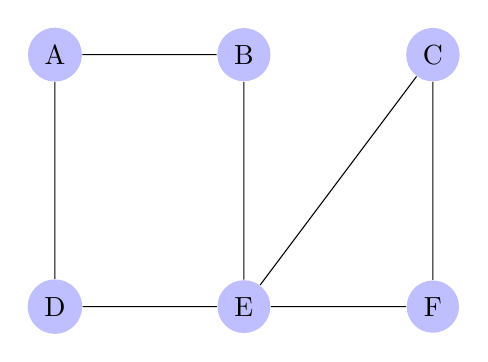
\begin{tikzpicture}
[scale=.8,auto=left,every node/.style={circle,fill=blue!25}]
  \node (n6) at (3,2) {D};
  \node (n4) at (3,6) {A};
  \node (n5) at (6,2) {E};
  \node (n1) at (6,6) {B};
  \node (n2) at (9,2) {F};
  \node (n3) at (9,6) {C};
  \foreach \from/\to in {n6/n4,n5/n1,n2/n5,n2/n3,n1/n4,n6/n5,n5/n3}
    \draw (\from) -- (\to);
\end{tikzpicture}
\caption{Euler kreds} 
\label{euler_kreds}
\end{figure}

\noindent Et eksempel på en Eulerkreds i Figur \ref{euler_kreds} kan være: $A,B,E,C,F,E,D,A$


\begin{figure}[h]
\centering
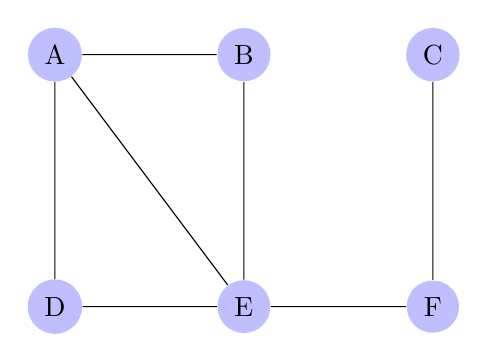
\begin{tikzpicture}
[scale=.8,auto=left,every node/.style={circle,fill=blue!25}]
  \node (n6) at (3,2) {D};
  \node (n4) at (3,6) {A};
  \node (n5) at (6,2) {E};
  \node (n1) at (6,6) {B};
  \node (n2) at (9,2) {F};
  \node (n3) at (9,6) {C};
  \foreach \from/\to in {n6/n4,n5/n1,n2/n5,n2/n3,n1/n4,n6/n5,n4/n5}
    \draw (\from) -- (\to);
\end{tikzpicture}
\caption{Euler vej} 
\label{euler_vej}
\end{figure}

\noindent Et eksempel på en Eulervej i Figur \ref{euler_vej} kan være: $A,B,E,D,A,E,F,C$\\

\noindent Der eksiserer ikke en Eulerkreds i alle grafer.
For at der kan eksisere en Eulerkreds i en sammenhægende multigraf skal Sætning \ref{Eulerkreds_multigraf} gælde. 

\begin{thm}\label{Eulerkreds_multigraf}
En sammenhængende multigraf med mindst to knuder, har en Eulerkreds hvis og kun hvis, hver knude er af lige grad.
\end{thm}

\begin{proof} 
Først bevises sammenhængen den ene vej. 
En kreds begynder i en knude $a$ og fortsætter langs en kant, som er incident med $a$, til en ny knude $b$. 
Denne kant kaldes $\lbrace a,b \rbrace$, kanten bidrager med 1 til $deg(a)$. 
Hver gang kredsen passerer gennem en knude, tilføjes 2 til graden af denne knude. 
Til sidst ender kredsen tilbage i $a$, og bidrager igen med 1 til $deg(a)$.
Hele graden af hver knude opnåes, da alle kanter skal passeres.  
Derfor må $deg(a)$ være lige og graden af hver knude må også være lige.  

Nu bevises sammenhængen den anden vej. 
For at finde en Eulerkreds i en sammenhægende multigraf  G, som opfylder at graden af hver knude er lige, tages først udgangspunkt i en tilfældig underkreds i grafen.
Denne underkeds starter i en knude $a$, hvorfra en simpel vej dannes ved at bevæge sig rundt i grafen. 
Dette forsætter indtil man når en knude hvor man ikke kan komme videre, fordi alle incidente kanter allerede er en del af den den simple vej, som nu er blevet til en kreds. 
Hvorefter et H indførers, som er lig med G, undtagen kanterne i den tilfældige underkreds.
Alle knuder i grafen vil stadig være af lige grad.
Fordi de fjernede kanter danner en kreds, må de dermed fjerner et lige tal fra graden af en knuder, eller en knude vil blive isoleret.
Så dannes en ny underkreds i H, som starter i et endepunkt i den tidligere underkreds.
Fordi grafen er sammenhængende vides det at den nye underkreds kan forbindes med en tidligere underkreds. 
Kanter i den nye underkreds fjernes fra H. 
Samtidig sættes de to underkredse sættes sammen til én kreds.
Denne procedure forsættes indtil der ikke er flere kanter i H.
Da må der være dannet en Eulerkreds. 
\end{proof} 
 
Proceduren kan ses i Algoritme \ref{algoritme_euler}.
Der findes også andre algoritmer, som kan finde Eulerkredse i en graf, men disse bliver ikke nævnt i dette projekt.\\
  

\begin{algorithm}
\caption{Eulerkredse}
\label{algoritme_euler}
\textbf{procedure} Euler(G: sammenhængende multigraf med knuder af lige grad)\\
$kreds:=$ en kreds i G der begynder i en vilkårlig knude med kanter, der danner en kreds.\\
$H:= G$ med kanterne fra $kreds$ fjernet\\
\textbf{når} $H$ har kanter\\
$\-$ $\-$ $\-$ $\-$ $\-$ $\-$
$underkreds:=$ en kreds i $H$, der begynder i en knude $v$ i $H$, som også er et endepunkt af en kant i $kreds$ \\ 
$\-$ $\-$ $\-$ $\-$ $\-$ $\-$
$H:=$ $H$ uden kanterne af $underkreds$ samt alle isolerede knuder fjernet \\
$\-$ $\-$ $\-$ $\-$ $\-$ $\-$
$kreds:=$ $kreds$ med $underkreds$ indsat \\ 
\textbf{retuner} $kreds$ ($kreds$ er en Eulerkreds)
\end{algorithm}

\noindent Hvis der ikke findes en Eulerkreds i en graf, kan der godt eksistere en Eulervej. 
Sætning \ref{Eulervej_multigraf} fortæller hvornår der findes en Eulervej. 

\begin{thm} \label{Eulervej_multigraf}
En sammenhængende multigraf graf G har en Eulervej, men ikke en Eulerkreds, hvis og kun hvis den har præcist to knuder af ulige grad.  
\end{thm} 

\begin{proof}
Først bevises sammenhængen den ene vej. 
Antag at en sammenhængende multigraf G har en Eulervej fra $a$ til $b$, men ikke en Eulerkreds. 
Den første kant som passeres på vejen bidrager med 1 til $deg(a)$. 
Hver gang vejen passerer knuden $a$ vil 2 tilføjes til $deg(a)$. 
Den sidste kant på vejen bidrager 1 til graden af endepunktet for vejen, $deg(b)$. 
Ligesom for $a$, kan vejen krydse $b$. 
Hver gang dette måtte ske tilføjes 2 til graden af $b$. 
Resultatet bliver, at $a$ og $b$ altid vil være af ulige grad. 
Alle andre knuder på vejen vil være af lige grad, fordi at 2 tilføjes til graden af en knude, hver gang en knude passeres.  

Nu bevises sammenhængen den anden vej.
Antag at $a$ og $b$ er de eneste knuder af ulige grad. 
Hvis en kant $\lbrace a,b \rbrace$ tilføjes til G, vil alle knuder i grafen være af lige grad. 
Så gælder Sætning \ref{Eulerkreds_multigraf}, og der vil være en Eulerkreds i G. 
Fjernes kanten $\lbrace a,b \rbrace$ igen vil der være en Eulervej. 
\end{proof}

\section{Hamiltonkredse}
En anden type kreds er en Hamiltonkreds. 
En Hamiltonkreds er en kreds som går gennem hver knude i grafen én gang. På samme måde kan der også eksistere en hamilton vej, som er en vej der går gennem hver kant i en graf én gang. 

\begin{defn} \label{hamiltion_defn}
En Hamilton vej er en simpel vej i en graf G, som går gennem hver knude én gang.
En simpel kreds i en graf G, som går gennem hver knude én gang kaldes en Hamiltionkreds.
\end{defn}

\begin{exmp}
Eksempler på en Hamiltionkreds og en Hamiltionvej kan ses her: \\

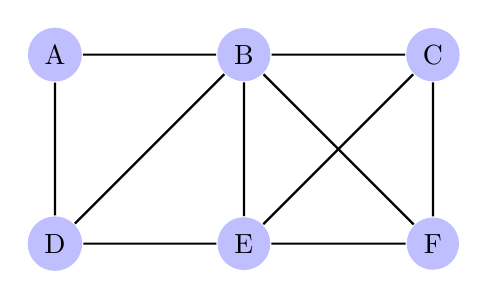
\begin{tikzpicture}
[thick,scale=.8,auto=left,every node/.style={circle,fill=blue!25}]
  \node (n6) at (3,2) {D};
  \node (n4) at (3,5) {A};
  \node (n5) at (6,2) {E};
  \node (n1) at (6,5) {B};
  \node (n2) at (9,2) {F};
  \node (n3) at (9,5) {C};
  \foreach \from/\to in {n6/n4,n4/n1,n6/n1,n6/n5,n1/n3,n1/n2,n1/n5,n5/n2,n5/n3,n3/n2}
    \draw (\from) -- (\to);
\end{tikzpicture}


\noindent Et eksempel på en Hamiltionkreds i grafen kan være: $A,B,F,C,E,D,A$\\
Et eksempel på en Hamiltionvej kan være: $A,D,B,C,F,E$
\end{exmp}

Der kendes ikke en simpel måde til at bestemme om der findes en Hamiltionkreds i en graf, ligesom der gør for en Eulerkreds. 
Der findes dog flere sætningerne der kan give en ide om eksistensen af en hamiltonkreds.
Den første sætning er Diraks sætning.

\begin{thm} \label{diracs_thm}
\textbf{Diracs Sætning:} 
Hvis G er en simpel graf med $n$ knuder, og $n\geq3$, så graden af hver knude i G er mindst $n/2$. 
Så har G en Hamiltionkreds.  
\end{thm}



En anden sætning, der minder meget om Diraks, er Ores' sætning.

\begin{thm} \label{diracs_thm}
\textbf{Ores Sætning:} 
Hvis G er en simpel graf med $n$ knuder, og $n\geq3$, så\\ $deg(u)+deg(v)\geq n$ for hvert par af ikke tilstødende knuder $u$ og $v$ i G. 
Så har G en Hamiltionkreds. 
\end{thm}

Derudover gælder det også, at der ikke kan eksistere en hamiltonkreds i en graf med en knude, der har graden 1. 
Disse to sætninger fortæller, hvornår der helt sikkert eksisterer en hamiltonkreds, men en hamiltonkreds kan godt eksistere uden at opfylde sætningerne. 

\begin{exmp}
I Figur \ref{pentagon} ses en graf der indeholder en hamiltonlkreds.
Grafen overholder ikke Diracs Sætning, fordi $n=5$, mens graden af hver kant i grafen er $2$, hvilket er mindre end $n/2$.
Grafen overholder heller ikke Ores' Sætning, da summen af to knuders grader aldrig kan give et resultat større end $4$, hvilket er mindre end $n$.

\begin{figure}
\centering

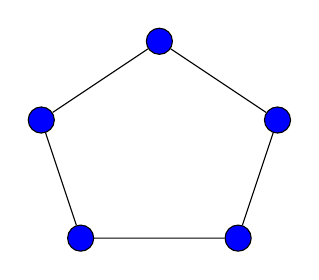
\begin{tikzpicture}[every node/.style={draw,shape=circle,fill=blue}]
\path (0,0) node (p0) {}
(-1.5,-1) node (p1) {}
(-1,-2.5) node (p2) {}
(1,-2.5) node (p3) {}
(1.5,-1) node (p4) {};
\draw (p0) -- (p1)
(p0) -- (p1)
(p0) -- (p4)
(p1) -- (p2)
(p2) -- (p3)
(p3) -- (p4);
\end{tikzpicture}
\caption{Hamiltonkreds i en graf med 5 knuder}
\label{pentagon}
\end{figure}

\end{exmp}

Det gælder i øvrigt, at jo flere kanter en graf har, jo større er sandsynligheden for at der eksisterer en hamiltonkreds. 